\documentclass[12pt]{extarticle}


\usepackage[pdftex]{graphicx}
\usepackage{float}
\usepackage{textcomp}
\usepackage[utf8]{inputenc}
\usepackage{hyperref}
\usepackage{float}
\usepackage{longtable}


\title{\textbf{SDN Overlay Network with VCL and \\Open vSwitch}}
\date{\today}
%Add your name in place of your handle
\author{\textbf{Team 9} \\Kushagra Mishra : Lead\\
B Shravan Achar : Vice Lead \\ Yogesh Lele \\ Muchen Zhang \\ Gokkulasudan Rathnakumar\\ \textbf{Computer Science Department} \\\textbf{NC State University}}


\begin{document}

\maketitle
\pagebreak

%TODO : independent index (aka ToC) (After completion of the report) for pages, graphs, tables.
%TODO : Each section of a new page after the completion of the report.
% list full names of all team members
\newpage         

\section{Abstract}
%{The infrastructure basically contains compute, storage and networking hardware. ---- Can we add HPC compute nodes as well}
Apache Virtual Computing Lab (VCL) is an open-source system used to dynamically provision and broker remote access to a dedicated compute environment for an end-user \cite{vcl}\cite{schaffer2009ncsu}. Setting up and maintaining VCL for a large institution like NCSU, requires large scale infrastructure. The infrastructure basically contains compute, storage and networking hardware. Managing a large virtual environment at scale grows in complexity as demand for VCL services increase. Software-defined networking (SDN) helps network administrators to easily configure networking devices in a dynamic environment, where requirements are changed on a regular basis. Currently, VCL uses Linux bridges over Kernel-based Virtual Machine (KVM) to communicate between VMs. The project aims to replace this infrastructure and use Open vSwitch(OVS) instead. With OVS running on all networking devices, it will be possible to control them using a SDN controller. This will ease the process of configuring multiple networking devices.

\pagebreak
\tableofcontents
\pagebreak
\listoffigures
\listoftables
\pagebreak
%Guys, we should add this below section

\section{Introduction}
Apache Virtual Computing Lab (VCL) is a free and open source cloud computing platform which provides custom compute resources on demand to its users \cite{vcl}\cite{schaffer2009ncsu}. These compute resources are provisioned to users in a virtualized environment. Virtualized networks or overlay networks are networks built on top of another(physical or virtual) network. Currently, the VCL uses Linux bridges to connect the VMs to the host’s physical networks. This project aims to replace those bridges with Open vSwitches and create an overlay network.

More about Apache VCL can be found in appendix \ref{apachevcl}.

% The compute environment can vary according to the user's requirement. The VCL platform can accommodate requirements ranging from simple virtual machines to cluster of physical machines running HPC(high performance computing) applications. Using VCL a user can provision several types of computer resources such as bare-metal machines, VMs hosted on hypervisors and traditional lab computers.

% The VCL environment also provides a front-end to facilitate the users to make reservations for custom computer resources. 



\subsection{Problem Statement}

\textbf{\emph{To create an SDN Overlay Network on VCL Sanboxes using Open vSwitch.}}
\\
\\
The current VCL network architecture faces two major problems:
\begin{enumerate}
    \item KVM hypervisors in the VCL infrastructure use linux bridges to connect to guest virtual machines. Use of linux bridges limits flexibility in network management. In particular, any new service on the linux bridges involves recompiling the bridge module.
    \item Further, in the current infrastructure, the "management" domain is restricted to a single KVM hypervisor. Virtual machines running on one KVM hypervisor form a local isolated network.
\end{enumerate}
  %stop writing need to upload who is this ?: This is Shravan.
  This project is aimed to modify this architecture by replacing the linux bridges with Open vSwitch bridges and interconnecting these bridges across multiple KVM hypervisors to improve manageability, configurability and flexibility of the VCL network.  

% This project involves configuring several KVM hypervisors within VCL to use Open vSwitch and VxLAN protocol to establish a SDN overlay network among the VCL nodes. 
% After establishing the overlay network, an openflow controller needs to be added to the SDN overlay. This provides a more complex control of the network. VCL sandboxes will be used to effectively establish a small VCL cluster running within the NCSU production VCL system.

% Currently, the KVM hypervisors are using Linux bridges to connect the VMs to the host’s physical networks. This project would replace those bridges with Open vSwitches.  Additionally, tunnels between the hypervisors would be created to establish a single private network for the project VCL cluster. After the private network has been created a single management node will be used to provision VMs on all the VCL sandboxes.

\subsection{Motivation}

In the present VCL environment, suppose a user wants to configure network for 10 VCL sandboxes (analogous to single tenant having VMs spanning across multiple data centers). The user will have to access each sandbox to manage or make changes to the network configuration. This is cumbersome and also takes a lot of time. An overlay network with a centralized controller provides a fine-grained control of the network. This results in a VMs-only virtual network across multiple sandboxes with a single management point. Such an overlay network enables cloud administrators to effectively manage mutliple VCL nodes to establish a small VCL cluster running within the NCSU production VCL system. 

\subsection{Issues}
% The networking of VCL sandboxes require 
\begin{enumerate}
    \item Libvirt does not attempt to manage the openvswitch bridge interface. So, no iptables rules, IP addresses, or DHCP/DNS services are added to ovs bridges by libvirt. All of these services must be added to it manually. 
    \item VxLAN encapsulation increases the packet size. Since the MTU of the network is 1500, VxLAN packets get fragmented and ultimately dropped. Due to this, it is observed frequently that ssh packets originating from management node of the master destined to the slave host get dropped and the SSH connection fails.
    \item Every sandbox has a maximum of 4 VMs. The MAC \& IP addresses of these 4 VMs match the MAC \& IP addresses of VMs in another sandbox. Because of this, more than a combined total of 4 VMs can not be brought up on two sandboxes put together without changing the MAC addresses of VMs. IP addresses, however, can be assigned differently by running a single DHCP server but the MAC addresses will have to be modified. Modifying MAC addresses involve modifying the VMs XML source file, which is out of scope for this project.
\end{enumerate}

% \subsection{Environment}

\section{Requirements}
\subsection{Functional Requirements}
\begin{enumerate}
    \item To replace the Linux bridge with open vSwitch on KVM inside a VCL Sandbox 2.4.2. After the bridge has been replaced, VCL should be able to provision VMs on the hypervisor, as it did before changing to Open vSwitch. Also, the networking changes should be persistent across reboots.
    \\
    \textbf{Sub requirements:}
    \begin{enumerate}   
        \item Install OvS
        \item Destroy all active VMs in the sandbox
        \item Add new OvS bridges for "nat" and "private" network
        \item Destroy and undefine the previous "nat" and "private" network configuration
        \item Define and load OvS "nat" and "private" network configuration
        \item Change firewall rules to allow traffic on OvS brige
        \item Configures DHCP for "nat" and "private" network
        
    \end{enumerate}

    \item To replicate the environment mentioned above on another VCL sandbox. 
    \\
    \textbf{Sub requirements:}
    \begin{enumerate}   
        \item Re-do steps as mentioned in functional-requirement 1.
        \item Destroy the management node.
    \end{enumerate}
    
    \item To establish a tunnel between the sandboxes running Open VSwitch and setup a private network using either VxLan tunnelling protocol.

    \item The management node on one VCL sandbox (master) should be able to provision VMs on all such sandboxes (slaves) over the earlier described private network. For this, a single common DHCP server running on the master sandbox must be used to provide IP addresses to VMs on all sandboxes. Users must still be able to connect to a reserved VM on any sandbox, as they did before the tunnel was established.
    
    \item To reconfigure the VCL sandboxes to use a single NAT host, preferably on the master sandbox. Thus, users should be able to connect to VMs on either host. However, all connections should be made through the public IP of only one host.

    
    % After completing step 1, you will have a single sandbox working that is using
    % Open vSwitch.  So, what will be the other endpoint for the tunnel described in
    % step 2?  You need to move part of what you have in step 3 to before step 2
    % (the part about replicating the environment).
    
    % You will need to modify DHCP for the private network.
    
    % Also, note that at this point you should have replaced both bridges in the
    % sandboxes with Open vSwitches, but you are only establishing a tunnel for the
    % private network.

        
    \item To install a SDN controller on one of the sandboxes to orchestrate Open vSwitches on all the sandboxes and police the traffic over the private and nat networks.
    
\end{enumerate}

\subsection{Non-Functional Requirements}
    \begin{enumerate}
        \item To analyze and mitigate known vulnerabilities and threats introduced by the migration to OvS.
        \item To analyze performance of the entire system after introducing SDN / OvS.
        \item To analyze scaling issues introduced by OvS and tunneling.
        \item To provide succinct documentation/scripts needed for a VCL administrator to replicate these setups without having to do additional research on what commands to run and how to configure things. 
    
    \end{enumerate}
    % Use of single NAT also limits scalability (port number / FDs). NAT host is overloaded, which might limit scalability
    % Possible solutions - Use load balancer in front of a NAT. Distributed NAT service.
    
\section{System Environment}
\begin{itemize}
    \item \textbf{VCL Sandbox 2.4.2}
    \newline
     A VCL Sandbox is a mini-cloud image containing collection of several VMs pre-configured. It also houses VCL\textquotesingle s Management Node daemon that is responsible for provisioning these VMs.
     
    \item \textbf{KVM/QEMU}
    \newline
    The de-facto hypervisor in Linux kernel coupled with QEMU for near native performance. VCL Sandbox internally uses KVM as its hypervisor for VM provisioning 
    
    \item \textbf{CentOS 7}
    \newline
    The operating system housing the KVM hypervisor 
    
    \item \textbf{Open vSwitch}
    \newline
    Virtual network switch that bridges VMs' public and private networks with the VCL private and public. Also provides scope for programmable reconfigurability and manageability
    
    \item \textbf{VxLan}
    \newline
    Overlay Networking protocol specialized for Data Center tunnelling. Ideal choice for handling overlay traffic across multiple Sandboxes
    
    \item \textbf{Open Daylight Controller}
    \newline
    An Software-Defined Network controller which can orchestrate the networking within VCL sandboxes remotely and programmatically providing flexibility and ease of management to administrators.
    
\end{itemize}


\section{Design}

This section describes the design of the entire system. 
KVM hypervisors in the current VCL system use linux bridges to communicate to the virtual machines running on top of them. Replacing the linux bridge with an Open vSwitch has certain advantages and disadvantages. They are enumerated below:
\\

\noindent
\textbf{Advantages:}
\begin{enumerate}
    \item Open vSwitch is highly programmable. Supports OpenFlow protocol.
    \item Enables flow routing. This provides greater flexibility in the number of match fields that can be defined for switching. 
    \item Specially designed for virtual environments. Supports all popular hypervisors including Xen and KVM. A migration to a different hypervisor does not involve changing the switching infrastructure
    \item Studies by Emmerich et.al. \cite{6968979} show that Open vSwitch offers better performance than native linux bridges
    \item Free and open-source
\end{enumerate}

\noindent
\textbf{Disadvantages:}
\begin{enumerate}
    \item Traditional linux images come up with linux bridges pre-installed. Open vSwitch functionality has to be installed separately
    \item Libvirtd does not manage ovs bridges whereas it can manage linux bridges. Ovs bridges will have to be managed manually.
\end{enumerate}

At the cost of installing and configuring the bridges, OvS improves flexibility and manageability of a virtual environment. These are the reasons why an important design choice in the project was to replace the linux bridges with OvS bridges.


\subsection{VCL Sandbox}

Figure \ref{fig:vcllinux} shows the current sandbox architecture being realised with linux bridges.
\begin{figure}[H]
\centering
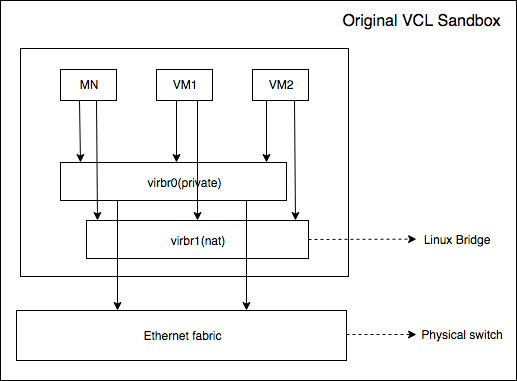
\includegraphics[width=0.9\textwidth]{vcl_linux_sandbox}
\caption{VCL sandbox with Linux Bridge}
\label{fig:vcllinux}
\end{figure}

The sandboxes have one dedicated VM for managing other VMs. This VM is called the 'management node' uses the linux bridge to communicate with other VMs. The number of nodes that one management node can manage is limited to one host.

\begin{figure}[H]
\centering
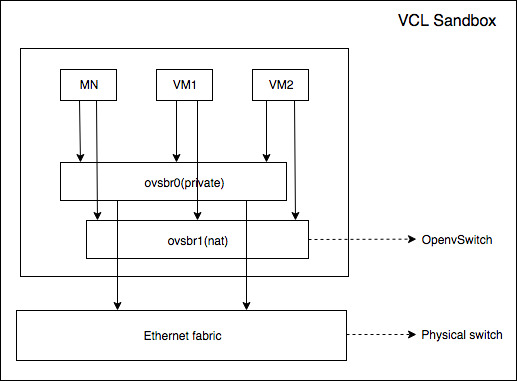
\includegraphics[width=0.9\textwidth]{vcl_ovs_sandbox}
\caption{VCL sandbox with Open vSwitch}
\label{fig:vclovs}
\end{figure}

The figure \ref{fig:vclovs} the linux bridges replaced with Open vSwitch bridges. 

\begin{figure}[H]
\centering
\includegraphics[width=0.9\textwidth]{vxlan_sandboxes}
\caption{VxLan tunnel between two VCL Sandbox}
\label{fig:vclvxlan}
\end{figure}

The ovs bridges are interconnected through a VxLan tunnel \cite{mahalingam2012vxlan}. A second design choice has been to use a suitable tunneling protocol to interconnect OvS switches
Some of the differences between VxLan and Geneve tunneling protocols are as follows:
\begin{enumerate}
    \item VxLan is a widely accepted protocol for network virtualization. Most switch hardware vendors support VxLan. 
    \item Geneve protocol is widely believed to be next-generation tunneling protocol due the flexibility it offers. However, lack of multivendor support for the protocol restricts its use in all network scenarios
    
\end{enumerate}
Modern data centers include a mix of hypervisor-based virtual machines, bare-metal workloads, and network services. All these components must be able to efficiently process packets and participate in an encapsulation protocol. Due to hardware interoperability and standardization, VxLan is better suited for network virtualization in data center environments

VxLan adds 50 bytes of header to an IP packet. This adds an overhead on applications such as SSH and Telnet where smaller packets are transmitted at short intervals (such as for each key stroke). Since, the interconnections are between two hosts, ssh/telnet use cases are not relevant in the current scenario.

\begin{figure}[H]
\centering
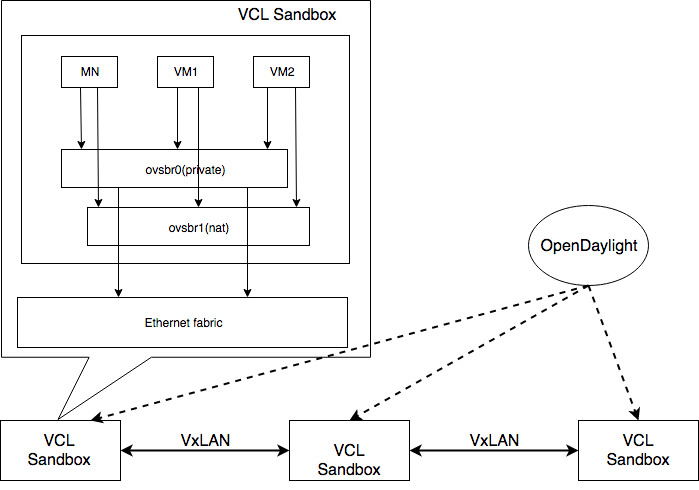
\includegraphics[width=0.9\textwidth]{Connected_vcl_sandboxes}
\caption{VCL Cluster with a single SDN Controller}
\label{fig:vclconnected}
\end{figure}

The figure \ref{fig:vclconnected} shows an SDN controller managing all the connected sandboxes. The SDN controller is only logically centralized whereas the controller process can run on any machine. Among the various controllers implementing the SDN concept, the choice to use Open Daylight is due to the following reasons:
\begin{enumerate}
    \item ODL is free and open source
    \item OpenDaylight project promises to standardize the northbound interface. This enables other controllers can leverage ODL to gain consistency across multiple vendors
    \item The implementation is enterprise ready. This has been seen in wide deployments of SDN systems with ODL controller such as CableLabs.
    \item ODL design is completely modular. It provides support for a wide range of services including NFV and IoT use cases.
\end{enumerate}


\section{Implementation}

This section describes implementation details of the project. 

\subsection{Installing OvS} \label{master_install_ovs}

OvS does not come pre-installed with stock Centos 7 machines and needs to be installed manually. There are many resources available online which provide step by step guide to install OvS. We followed one such article to configure OvS in our setup \cite{ovsinstall}. Appendix \ref{ovs_install}, provides details on step by step manual installation of OvS and using a script.

\noindent
There are three main functions which the script performs to install OvS \cite{ovs_script}:

\begin{enumerate}
    \item Install required packages for OvS: \textit{install\_ovs\_required\_packages()}
    \item Add user OvS: \textit{add\_new\_user("ovs")}
    \item Install OvS Packages: \textit{install\_ovs\_packages()}
\end{enumerate}


\subsection{Configuring OvS for master VCL Sandbox} \label{master_configure_vcl}
To configure Open vSwitch for a single VCL sandbox the following steps need to be followed: 
\begin{enumerate}
    \item Destroy the old "private" and "nat" bridge networks
    \item Create two new bridges for "private" as "ovsbr0" and "nat" as "ovsbr1"
    \item Create new OvS xml configuration file for each "private" and "nat" network
    \item Add new OvS bridge for both "private" and "nat" network
    \item Assign the network bridges IP 
    \item Define the new "private" and "nat" bridge network using the OvS xml configuration. 
    \item Start the new "private" and "nat" bridge network
    \item Change firewall rules for the new bridges (virbr0 $->$ ovsbr0 \& virbr1 $->$ ovsbr0)
    \item Configuring DHCP for master VCL Sandbox
    \begin{enumerate}
    \item Define a new DHCP configuration for "nat" and "private" network
    \item Define a new DHCP hostfile for "nat" and "private" network
    \item Define a new DHCP additional hosts file for "nat" and "private" network
    \item Load the DHCP configuration for "nat" and "private" network
    \end{enumerate}
\end{enumerate}

Appendix \ref{ovs_one_sandbox}, provides details on step by step manual configuration of OvS for a single sandbox.

\subsection{Replicate the setup for slave sandbox} 
To replicate the setup in slave sandbox, all the steps in section \ref{master_install_ovs} and section \ref{master_configure_vcl}. The following things need to kept in mind while configuring the slave sandbox:
\begin{itemize}
    \item DHCP should not be configured. There steps in section \ref{master_configure_vcl}, till item number 8 need to be followed.
    \item IP address of ovsbr0 and ovsbr1 should be different from master sandbox OvS brige IP address.
\end{itemize}

\subsection{Configuring VxLan tunnel}

VxLan tunnels need to be configured between the master and slave sandbox to create an overlay network. There are two tunnels which are created for "private" and "nat" network, through the public interface of master and slave sandbox. The following steps need to be followed to configure tunnels for the sandbox:
\begin{enumerate}
    \item Set up VxLan tunnel for "nat" network \cite{vxlan}.
    \item Set up VxLan tunnel for "private" network \cite{vxlan}.
    \item Add firewall rule in master to allow UDP packet at VxLan tunnel port from slave sandbox.
    \item Add firewall rule in slave to allow UDP packet at VxLan tunnel port from master sandbox.
    \item Change MTU size for all the interfaces to 1400.
\end{enumerate}
Appendix \ref{vxlan_config}, provides details on step by step manual configuring tunnel between master and slave sandbox.

\subsection{Adding slave as a virtual host}
The management node should be aware that it can provision VMs on another virtual host. To achieve this we need to add a virtual host using the VCL web interface. To add a virtual host the following steps need to be followed:

\begin{enumerate}
    \item Login to VCL web interface (master VCL sandbox management node)
    \item Go to Manage Computers tab $->$ Add new computer $->$ Add details of the slave sandbox, details in figure \ref{fig:vclvirtualhost}
    \item Go to virtual host tab $->$ configure host slave $->$ Add vms to the slave, details in figure \ref{fig:vclvm}
    \item Add firewall rule in slave to allow traffic from masters public IP address.
    \begin{verbatim}
    root \$ iptables -I INPUT -s <master_public_ip>/32 \
    -p tcp --dport 22 -j ACCEPT
    \end{verbatim}
    \item Add firewall rule in slave to allow traffic from masters private IP address.
    \begin{verbatim}
    root \$ iptables -I INPUT -s <master_private_ip>/32 \
    -p tcp --dport 22 -j ACCEPT
    \end{verbatim}
\end{enumerate}

The steps mentioned above call a SQL procedure, which adds a virtual host in the management node's database \cite{sqlprocedure}.


\subsection{Extra Script Features}
The script provides a default option to configure a single VCL sandbox with OvS switch. It performs the following function:
\begin{enumerate}
    \item Install packages required by OvS
    \item Fetch OvS tarball and install OvS
    \item Start the OvS service
    \item Add new OvS bridges for "nat" and "private" network
    \item Destroy and undefine the previous "nat" and "private" network configuration
    \item Define and load OvS "nat" and "private" network configuration
    \item Configures DHCP for "nat" and "private" network
\end{enumerate}

\begin{verbatim}
root \$ ovs_vcl.py --default
\end{verbatim}


\section{Results}
To-Do
\section{Verification and Validation}
%{The start up time for a host having Linux Bridges and Open v Switch bridges has not been validated. The reason is because we were provided with a pre booted up production machines to work on.}

%{Need to check the ping rate and external access to the VM}
\subsection{Functional Requirements V \& V}

\begin{center}


\begin{table}[H]
\begin{tabular}{||c  | p{0.5\linewidth} | p{0.5\linewidth} ||}
  % Please fix the alignment for the table
     \hline
     Req. No & Test Cases & Expected Result  \\
     \hline \hline
     1 & Bring up a new VM on the master sandbox either from CLI or virt-manager & VMs must be able to be provisioned the same way as before\\
     \hline
     1 & After the new VM is up, list the ports of ovs bridge and ping the private interface of the VM from the host & The VMs must attach themselves to the ovs bridge, and the ping test must pass \\
     \hline
     1 & Ping the eth1 interface (NAT) of the VM from the master host & The ping from the host must go through the ovs bridge \\
     \hline
     2 & Perform the same tests as the first functional requirement for new VMs on the second sandbox (called slave) & The behaviour must be consistent with the results in first functional requirement \\
     \hline
     3 & Perform reachability test from ovs bridges on master to the corresponding ovs bridges on the slave & Tunnels are considered to be set up correctly if the ping test is successful and traceroute shows the bridges as adjacent to each other \\
     \hline
     3 & Collect the output of arp on both hosts & The arp table must have entries for the other tunnel end point \\
    
     \hline
     4 & Bring down the VMs on both the sanboxes and bring them back up. Collect the output of ifconfig on both VMs & All private interfaces must have IP addresses in the same subnet and all nat interfaces must have IP addresses in the same subnet \\
     \hline
     4 & Bring down the central DHCP process. Bring down the VMs on both the sandboxes and bring them back up. Collect the output of ifconfig on both VMs & It is expected that no VMs will be assigned IP addresses and collecting ifconfig output would be impossible \\
     \hline
     4 & SSH into the management node of the master sandbox from both master and slave hosts & Since there is only one management node, SSH must take the user (root) to the same VM \\
     \hline
     4 & SSH into the management node of the slave sandbox from both master and slave hosts & Since there is only one management node, SSH into the slave sandbox must fail from both the hosts \\
     \hline 
     \end{tabular}
     \end{table}
     
     \begin{table}[H]

     \begin{tabular}{||c  | p{0.5\linewidth} | p{0.5\linewidth} ||}
     \hline
     4 & From the management node of the master sandbox, SSH into both master and slave sandboxes & Since the management node must be able to login to each sandbox to provision new VMs, SSH must go through \\
     \hline
     4 & Bring down all guest VMs. Bring up a new virtual machine on the slave sandbox & The VM must be successfully provisioned and it must be possible to SSH into the new VM from the management node \\
     \hline
     4 & Bring down all guest VMs. Bring up a new virtual machine on the master sandbox & The VM must be successfully provisioned and it must be possible to SSH into the new VM from the management node \\
     \hline
     5 & Collect the outputs of tcpdump on eth1 interfaces of both master and slave sandboxes. Ping www.google.com from the VM provisioned on the master sandbox & The output of tcpdump on master must show ICMP traffic from the VM, whereas the output of tcpdump on slave must not have this ping traffic \\
     \hline
    5 & Repeat the same experiment as above, but this time ping www.google.com from the VM provisioned on the slave sandbox & The ping traffic must still go through the eth1 interface of the master sandbox, thereby validating the use of a single NAT \\
     \hline
    6 & Ping from private interface of one VM to the private interface of another VM & This ping must fail since the VMs were reserved individually and hence isolation must be maintained\\
    \hline
    6 & Ping from the private interface of management node to the private interfaces of both the guest VMs & The ping traffic must successfully complete \\
    \hline
    6 & Ping from the nat interface of one VM to the nat interface of another VM & This ping must successfully complete. Although reachability must be through the public network and not through the configured tunnel between the bridges \\
    \hline
    6 & Ping from the nat interface of management node to the nat interface of both the guest VMs & This ping must successfully complete. The reachability must be through the configured tunnel between the ovs bridges \\
    \hline
    6 & Create reservations for 4 VMs & All the reservations must successfully complete. Output of 'virsh list' command on both master and slave sandboxes must show 2 VMs each \\
    \hline
\end{tabular}
\caption{Functional Requirements}
\label{table:func_vv}
\end{table}
\end{center}

\begin{center}
\begin{table}[H]
\subsection{Non-Functional Requirements V \& V}
\begin{tabular}{||c  | p{0.5\linewidth} | p{0.5\linewidth} ||}
  % Please fix the alignment for the table
     \hline
     Req. No & Verification & Validation  \\ 
     \hline \hline
     1 & Perform a flow table overflow attack on the controller & Analyze the system's behaviour on different active and inactive times for flow table entries \\
     \hline
     2 & Create a small payload, high packet-rate traffic flow targetted at the ovs bridge & SDN systems with a software switch are known to under-perform when dealing with high-packet rate and short payloads. Analyze the system behaviour under this scenario \\
     \hline
     4 & Provide the completed documentation to a volunteer from class & The volunteer must be able to provision new VMs and apply network policies through the controller with the help of provided documentation alone \\     
    \hline
\end{tabular}
\caption{Non-Functional Requirements}
\label{table:nonfunc_vv}
\end{table}
\end{center}

\section{Schedule and Personnel}
%{Configuring Open vSwitch with the help of pm modules}
%{DHCP configuration}
%{NAT Host Configuration}
%{Floodlight Setup}
%{VxLan Setup to allow tunnelling}
%{Documetation}

\subsection{Task Allotment}


% \captionof{table}{Task Allotment} \label{tab:task} 
\begin{center}
\begin{table}[H]
 \begin{tabular}{||l | c | c ||} 
 \hline
 Task & Owner & Backup \\ [2ex] 
 \hline\hline
  Configuring Open vSwitch & Shravan & Yogesh  \\
  \hline
  Replicate Open vSwitch environment in another sandbox & Gokkul & Muchen  \\ 
  \hline
  Establish tunnel between VCL Sandbox(VxLan) & Kushagra & Gokkul  \\ 
  \hline
  Configure all hosts in VxLan to use a single NAT & Muchen & Kushagra  \\ 
  \hline
  Configure all hosts in VxLan to use a single DHCP & Shravan & Yogesh  \\ 
  \hline
  Installing floodlight controller and integrating it with VCL & Yogesh & Kushagra  \\ 
 \hline
 \end{tabular}

\caption{Task Allotment}
\label{table:task}
\end{table}
\end{center}

\subsection{Milestones}
\begin{center}
\begin{table}[H]
% \captionof{table}{Milestones} \label{tab:milestones}
 \begin{tabular}{||l | c | c ||} 
 \hline
 Milestone & ETA & Status \\ [2ex] 
 \hline\hline
  Configuring Open vSwitch & 03/20/2017 & Completed  \\
\hline
  Replicate Open vSwitch environment in another sandbox & 03/29/2017 & Completed  \\
  
   \hline
  Installing opendaylight controller  & 04/05/2017 & Completed  \\ 
  \hline
  Establish tunnel between VCL Sandbox(VxLan) & 04/15/2017 & Completed  \\ 
 
  \hline
  Configure all hosts in VxLan to use a single NAT & 04/17/2017 & Completed  \\ 
  \hline
  Configure all hosts in VxLan to use a single DHCP & 04/19/2017 & Completed  \\ 
  \hline
   Integrating the open daylight controller it with VCL & 04/21/2017 & Completed  \\ 
 \hline
 \end{tabular}
\caption{Milestones}
\label{table:milestone}
\end{table}
\end{center}

\bibliographystyle{ieeetr}
\bibliography{main}

%Things to be added 
\section{Appendix}
\subsection{Terminology}
\begin{enumerate}
    \item \textbf{KVM - Kernel Virtual Machine}
     \newline
    Kernel-based Virtual Machine (KVM) is a virtualization infrastructure for the Linux kernel that turns it into a hypervisor. It provides a loadble kernel module for the users that underlying architecture specific e.g. Intel, AMD
    
    \item \textbf{SDN - Software Defined Networking}
    \newline
    Software Defined Networking is an approach to computer networking provides separation of control and data plane in a forwarding device and facilitates programmability to initialize, control, change, and manage network behavior dynamically and remotely.
    
    \item \textbf{VCL - Virtual Computing Lab}
    \newline
    Apache VCL is a free and open-source cloud computing platform with the primary goal of delivering dedicated, custom compute environments to users.
    
    \item \textbf{OVS - Open vSwitch}
    \newline
    Open vSwitch is a production quality, multilayer virtual switch. It is designed to enable massive network automation through programmatic extension, while still supporting standard management interfaces and protocols
    
    \item \textbf{NAT - Network Address Translation}
    \newline
    Network address translation (NAT) is a method of remapping one IP address space into another by modifying network address information in Internet Protocol (IP) datagram packet headers while they are in transit across a traffic routing device. The technique was originally used for ease of rerouting traffic in IP networks without readdressing every host.
    
    \item \textbf{Sandbox - Virtual Computing Lab Sandbox}
    \newline
    A VCL Sandbox is a mini-cloud image containing collection of several VMs pre-configured. It also houses VCL\textquotesingle s Management Node daemon that is responsible for provisioning these VMs.  
    
\end{enumerate}
\pagebreak
\subsection{Apache Virtual Computing Lab} \label{apachevcl}
Apache VCL is an open-source implementation of a secure production-level on-demand services-oriented technology for wide-area access to solution based on real and virtualized resources, including computational, storage, networking, and software resources. It offers capabilities that are very flexible and diverse ranging from offering infrastructure-as-a-service, platform-as-a-service, software-as-a-service, also provides applications-as-a-service and more recently cloud-as-a-service and different combinations of those, to individual and group IT services, including HPC services.

The baseline service of VCL is provisiong of bare-metal and virtualized resources and extended services encompass PaaS and SaaS. VCL also allow users to install it and adapt it to their needs. A typical user accesses VCL through a Web interface, which after appropriate authentication and authorization steps, presents the user with a set of menu options. A number of additional VCL management functions are available for users with different levels of administrative privileges. In the Web interface, a user can select a particular environment of interest and request it of a given period of time. The image or image environment is loaded, for the duration requested, on either implicit automatically assisgned resources or on an explicit set of resources. VCL also has a network-oriented API that allows remote applications, middleware, and operating systems to access the same functionality through a publishable service. This allows automatic augmentation of end-user needs and seamless addition of resources provided the end-user platform is configured to do so.

\begin{figure}[H]
\centering
\includegraphics[width=1\textwidth]{vcl_arch}
\caption{VCL sandbox with Open vSwitch}
\label{fig:vclarch}
\end{figure}

The top-level architecture of VCL is illustrated in figure \ref{fig:vclarch}. There are seven major groups of components:
\begin{enumerate}
    \item end-user access interface
    \item authentication service
    \item VCL manager that manages user requests
    \item VCL database
    \item node manager that manages local installation resources and loads VCL images
    \item image repository
    \item computational, storage, and networking resources
\end{enumerate}

The VCL architecture abstracts resources at several levels: at the application and OS level via images and hypervisors, at the hardware location level (via VCL manager and nodes), and at the network level (via virtual networks, VLANs, VPNs).

\subsection{Implementation Details: Code \& Configuration Instructions}

The section contains code, configuration instructions and other detail relevant to the implementation of the project.

\subsubsection{Installing OvS} \label{ovs_install}

\begin{enumerate}
    \item \textbf{Manual Configuration}
    
\textbf{Fetch packages required by Open vSwitch, Run these commands as root user:}
\begin{verbatim}
root \$ yum -y install wget gcc make python-devel openssl-devel
kernel-devel graphviz kernel-debug-devel autoconf automake 
rpm-build redhat-rpm-config libtool
\end{verbatim}
\noindent
\textbf{Add a new user: }

\begin{verbatim}
root \$ adduser ovs
\end{verbatim}
\noindent
\textbf{Switch to user ovs:}

\begin{verbatim}
root \$ su - ovs
\end{verbatim}
\noindent
\textbf{As user ovs, generate the rpm file:}

\begin{verbatim}
ovs \$ mkdir -p ~/rpmbuild/SOURCES
ovs \$ wget http://openvswitch.org/releases/openvswitch-2.5.2.tar.gz
ovs \$ cp openvswitch-2.5.2.tar.gz ~/rpmbuild/SOURCES/
ovs \$ tar xfz openvswitch-2.5.2.tar.gz
ovs \$ rpmbuild -bb --nocheck openvswitch-2.5.2/rhel/openvswitch.spec
ovs \$ exit
\end{verbatim}

\noindent
\textbf{Create open vSwitch configuration directory, run as root user:}

\noindent
\begin{verbatim}
root \$ mkdir /etc/openvswitch
\end{verbatim}

\noindent
\textbf{Install the rpm package}
\begin{verbatim}
root \$ yum localinstall /home/ovs/rpmbuild/RPMS/x86_64/openvswitch-2.5.2-1.x86_64.rpm
\end{verbatim}

\noindent
\textbf{Start Open vSwitch service:}
\begin{verbatim}
root \$ systemctl start openvswitch.service
\end{verbatim}

\noindent
\textbf{Enable Open vSwitch at boot time:}
\begin{verbatim}
root \$ chkconfig openvswitch on
\end{verbatim}

\noindent
\textbf{Check if ovs command line tools are installed:}
\begin{verbatim}
root \$ ovs-vsctl --version
ovs-vsctl (Open vSwitch) 2.5.2
Compiled Apr 18 2017 00:21:19
DB Schema 7.12.1
\end{verbatim}

\item \textbf{Configure using Script}

Running the following command will install the OvS along with its required packages.
\begin{verbatim}
root \$ ovs_vcl.py --install-ovs   
\end{verbatim}
\noindent
The script runs all the commands mentioned in section \ref{ovs_install} in the given order.
\end{enumerate}


\subsubsection{Configuring OvS for a single VCL Sandbox} \label{ovs_one_sandbox}

\begin{enumerate}
\item \textbf{Manual Configuration}

\noindent
\textbf{Destroy the old "private" and "nat" bridge networks:}
\begin{verbatim}
root \$ virsh net-destroy private
root \$ virsh net-destroy nat
\end{verbatim}

\noindent
\textbf{Undefine the old "private" and "nat" bridge networks:}
\begin{verbatim}
root \$ virsh net-undefine private
root \$ virsh net-undefine nat
\end{verbatim}

\noindent
\textbf{Create a new bridge for "private" network:}
\begin{verbatim}
root \$ ovs-vsctl add-br ovsbr0
\end{verbatim}

\noindent
\textbf{Create a new bridge for "nat" network:}
\begin{verbatim}
root \$ ovs-vsctl add-br ovsbr1
\end{verbatim}


\noindent
\textbf{Create a new OvS xml configuration file for "private" network:}
\begin{verbatim}
<network>
  <name>private</name>
  <forward mode='bridge'/>
  <bridge name='ovsbr0'/>
  <virtualport type='openvswitch'/>
</network>
\end{verbatim}

\noindent
\textbf{Create a new OvS xml configuration file for "nat" network:}
\begin{verbatim}
<network>
  <name>nat</name>
  <forward mode='bridge'/>
  <bridge name='ovsbr1'/>
  <virtualport type='openvswitch'/>
</network>
\end{verbatim}

\noindent
\textbf{Assign IP to bridge:}
\begin{verbatim}
root \$ ifconfig ovsbr0 192.168.100.10
root \$ ifconfig ovsbr1 192.168.200.10
\end{verbatim}

\noindent
\textbf{Define net "private" network:}
\begin{verbatim}
root \$ virsh net-define <private_ovs_configuration_file.xml>
\end{verbatim}

\noindent
\textbf{Define net "nat" network:}
\begin{verbatim}
root \$ virsh net-define <nat_ovs_configuration_file.xml>
\end{verbatim}

\noindent
\textbf{Start new "private" network:}
\begin{verbatim}
root \$ virsh net-start private
\end{verbatim}


\noindent
\textbf{Start new "nat" network:}
\begin{verbatim}
root \$ virsh net-start nat
\end{verbatim}


\noindent
\textbf{Enable new "private" network on startup:}
\begin{verbatim}
root \$ virsh net-autostart private
\end{verbatim}

\noindent
\textbf{Enable new "nat" network on startup:}
\begin{verbatim}
root \$ virsh net-autostart nat
\end{verbatim}

\noindent
\textbf{Define a new DHCP configuration for "nat" network}
\begin{verbatim}
root \$ cat >> /var/lib/libvirt/dnsmasq/nat.conf
strict-order
domain=nat
expand-hosts
pid-file=/var/lib/libvirt/network/nat.pid
except-interface=lo
bind-dynamic
interface=ovsbr1
dhcp-range=192.168.200.128,192.168.200.254
dhcp-no-override
dhcp-lease-max=127
dhcp-hostsfile=/var/lib/libvirt/dnsmasq/nat.hostsfile
addn-hosts=/var/lib/libvirt/dnsmasq/nat.addnhosts
\end{verbatim}
Assumptions:
\begin{enumerate}
\item The bridge(interface) associated with "nat" network is "ovsbr1".
\item The DHCP range available is 192.168.200.128 to 192.168.200.254.
\item The pid-file, dhcp-hostsfile and addn-hosts are defined at the path mentioned above.
\end{enumerate}

\noindent
\textbf{Define a new DHCP configuration for "private" network.}
\begin{verbatim}
root \$ cat >> /var/lib/libvirt/dnsmasq/private.conf
strict-order
domain=private
expand-hosts
pid-file=/var/lib/libvirt/network/private.pid
except-interface=lo
bind-dynamic
interface=ovsbr0
dhcp-option=3
dhcp-range=192.168.100.128,192.168.100.254
dhcp-no-override
dhcp-lease-max=127
dhcp-hostsfile=/var/lib/libvirt/dnsmasq/private.hostsfile
addn-hosts=/var/lib/libvirt/dnsmasq/private.addnhosts
\end{verbatim}
Assumptions:
\begin{enumerate}
\item The bridge(interface) associated with "private" network is "ovsbr0".
\item The DHCP range available is 192.168.100.128 to 192.168.100.254.
\item The pid-file, dhcp-hostsfile and addn-hosts are defined at the path mentioned above.
\end{enumerate}

\noindent
\textbf{Define a new DHCP hostfile for "nat" network}
\begin{verbatim}
root \$ cat >> /var/lib/libvirt/dnsmasq/nat.hostsfile
52:54:00:3d:85:f0,192.168.200.1
\end{verbatim}

\noindent
\textbf{Define a new DHCP hostfile for "private" network}
\begin{verbatim}
root \$ cat >> /var/lib/libvirt/dnsmasq/private.hostsfile
52:54:00:b8:33:d4,192.168.100.1
52:54:00:ae:cf:00,192.168.100.101
52:54:00:ae:cf:02,192.168.100.102
52:54:00:ae:cf:04,192.168.100.103
52:54:00:ae:cf:06,192.168.100.104
\end{verbatim}

\noindent
\textbf{Define a new DHCP additional hosts file for "nat" network}
\begin{verbatim}
root \$ touch /var/lib/libvirt/dnsmasq/nat.addnhosts
\end{verbatim}

\noindent
\textbf{Define a new DHCP additional hosts file for "private" network}
\begin{verbatim}
root \$ touch /var/lib/libvirt/dnsmasq/private.addnhosts
\end{verbatim}


\noindent
\textbf{Load the DHCP configuration for "nat"network}
\begin{verbatim}
root \$ /sbin/dnsmasq --conf-file=/var/lib/libvirt/dnsmasq/nat.conf \
--log-facility=/var/lib/libvirt/dnsmasq/nat.log
\end{verbatim}

\noindent
\textbf{Load the DHCP configuration for "private"network}
\begin{verbatim}
root \$ /sbin/dnsmasq --conf-file=/var/lib/libvirt/dnsmasq/private.conf \
--log-facility=/var/lib/libvirt/dnsmasq/private.log
\end{verbatim}

\end{enumerate}

\subsubsection{Configuring VxLan tunnel} \label{vxlan_config}

\begin{enumerate}


\item \textbf{Setting up Private Tunnel}
\noindent

\textbf{Create a VTEP interface on OvS bridge for private tunnel on master}
\begin{verbatim}
ovs-vsctl add-port ovsbr0 tun0 --set interface tun0 type=vxlan \
options:remote_ip=<slave_private_ip> options:key=123
\end{verbatim}

\noindent
\textbf{Create a VTEP interface on OvS bridge for private tunnel on slave}
\begin{verbatim}
ovs-vsctl add-port ovsbr0 tun0 --set interface tun0 type=vxlan \
options:remote_ip=<master_private_ip> options:key=123
\end{verbatim}


\item \textbf{Setting up Public("nat) Tunnel}
\textbf{Create a VTEP interface on OvS bridge for public tunnel on master}
\begin{verbatim}
ovs-vsctl add-port ovsbr1 tun1 --set interface tun1 type=vxlan \
options:remote_ip=<slave_public_ip> options:key=456
\end{verbatim}

\noindent
\textbf{Create a VTEP interface on OvS bridge for public tunnel on slave}
\begin{verbatim}
ovs-vsctl add-port ovsbr1 tun1 --set interface tun1 type=vxlan \
options:remote_ip=<master_public_ip> options:key=456
\end{verbatim}

\item \textbf{Add firewall rules for master sandbox}
\noindent
\begin{verbatim}
iptables -I INPUT -s <slave_ip>/32 -p udp -m udp --dport <vxlan_port> -j ACCEPT
\end{verbatim}

\item \textbf{Add firewall rules for slave sandbox}
\noindent
\begin{verbatim}
iptables -I INPUT -s <master_ip>/32 -p udp -m udp --dport <vxlan_port> -j ACCEPT
\end{verbatim}

\item \textbf{Change the MTU size for public and private interfaces and bridges in master and slave sandbox. Also, change it in any of the VMs (management node or others) which are provisioned}
\begin{verbatim}
ifconfig <interface> mtu 1400
\end{verbatim}

\end{enumerate}

\subsubsection{Adding Virtual Host}
\begin{figure}[H]
\centering
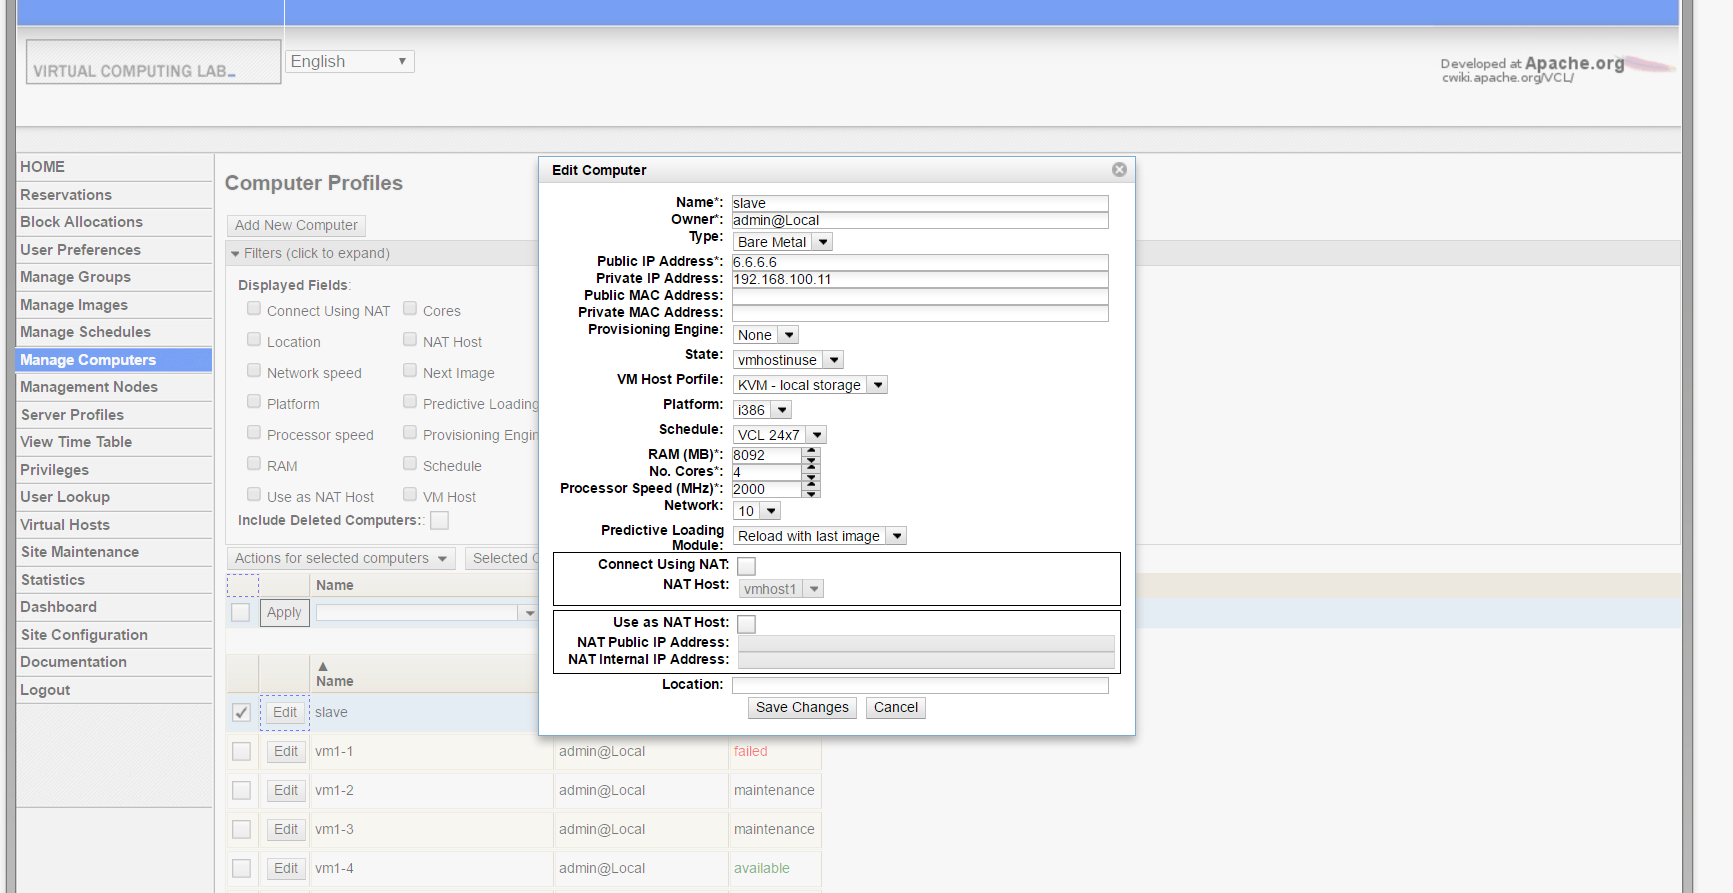
\includegraphics[width=0.9\textwidth]{add_computer}
\caption{Add virtual host}
\label{fig:vclvirtualhost}
\end{figure}

\begin{figure}[H]
\centering
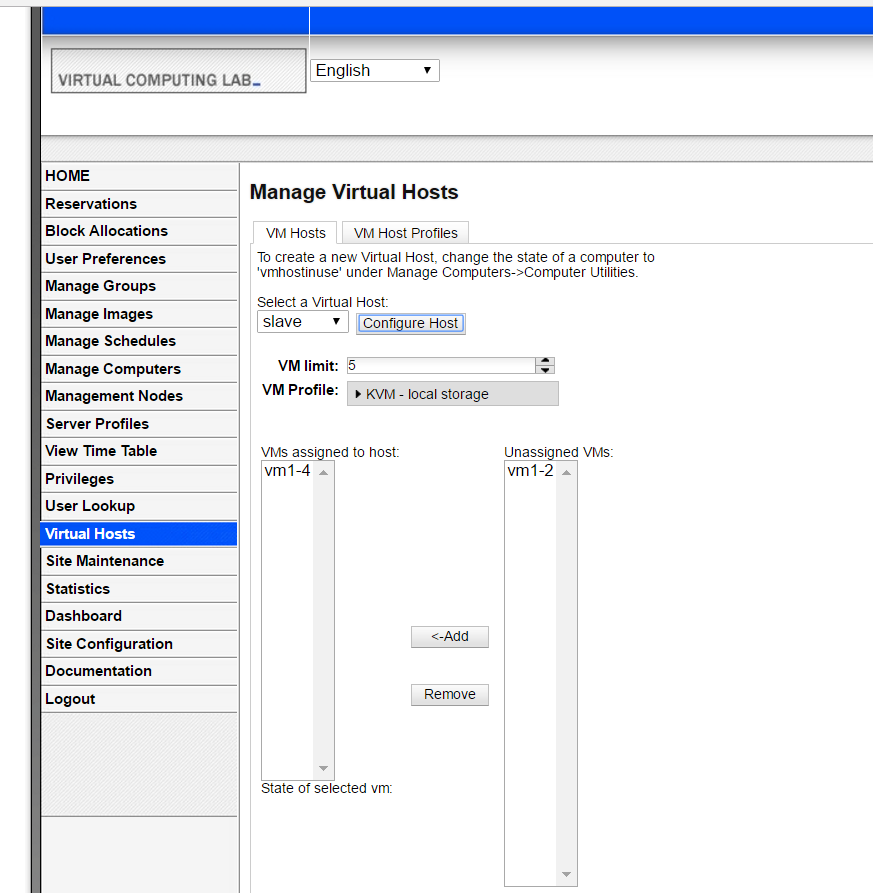
\includegraphics[width=0.9\textwidth]{add_virtualhost}
\caption{Add VMs to slave sandbox}
\label{fig:vclvm}
\end{figure}



\end{document}
